% Interaction terms and nonlinear trends

\begin{frame}{Consider}
    Consider an experiment that examines the impact of Vitamin C from two sources on the growth of teeth in Guinea pigs.
    \begin{itemize}
        \item Each Guinea pig was randomly assigned to one of two possible levels of each variable.
        \begin{itemize}
            \item \texttt{supp} indicates a supplement type for Vitamin C, with levels \texttt{VC} for ascorbic acid and \texttt{OJ} for orange juice.
            \item \texttt{dose} indicates the amount of Vitamin C, which takes values of either 1 or 2 mg.
        \end{itemize}
    \end{itemize}
The outcome is the tooth length of the Guinea pigs.
\end{frame}

\begin{frame}{Example}
    \begin{itemize}
        \item We want to build a regression model for these data.
        \item We start with the following model:
    \end{itemize}
    \[
        Y = \beta_0 + \beta_1 x_{supp} + \beta_2 x_{dose} + \epsilon
    \]
\end{frame}

\begin{frame}{Example}
    The model output is
    \begin{table}[h]
    \begin{tabular}{r rrrr}
        \hline
         & Estimate & Std. Error & t value & Pr($>|$t$|$) \\
        \hline
        (Intercept) & 14.8325 & 2.0319 & 7.30 & 0.0000 \\
        suppVC & -2.9250 & 1.2253 & -2.39 & 0.0222 \\
        dose & 6.3650 & 1.2253 & 5.19 & 0.0000 \\ 
        \hline
    \end{tabular}
    \end{table}
    Write the regression model for these data.
\end{frame}

\begin{frame}{Example}
    \begin{center}
        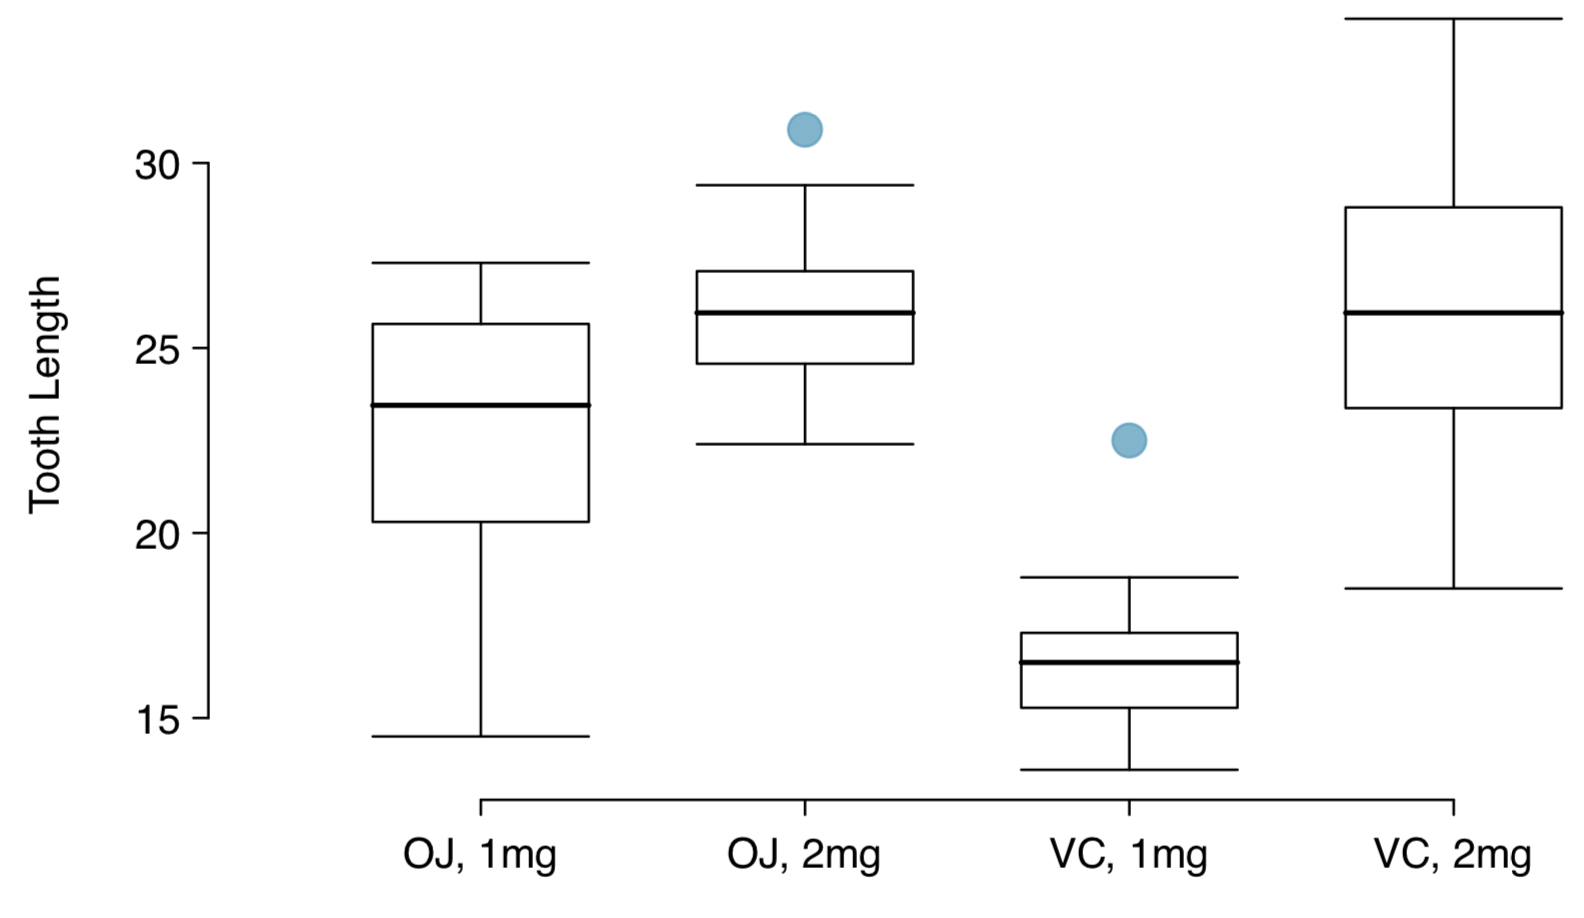
\includegraphics[width=4in]{images/toothbox.png}
    \end{center}
    Predict an outcome for each possible combination of variables. How do these means compare to the boxplots?
\end{frame}

\begin{frame}{Example}
    For this model,
    \begin{itemize}
        \item R$^2 = 0.5553$
        \item R$^2_{adj} = 0.5183$ 
    \end{itemize}
    
    \vspace{12pt}When we built our model, we assumed that the effects of the supplement and dose are independent. 
    \begin{itemize}
        \item What if this isn't the case?
        \item Can we improve the model?
    \end{itemize}
\end{frame}

\begin{frame}{Interactions}
    \centering
    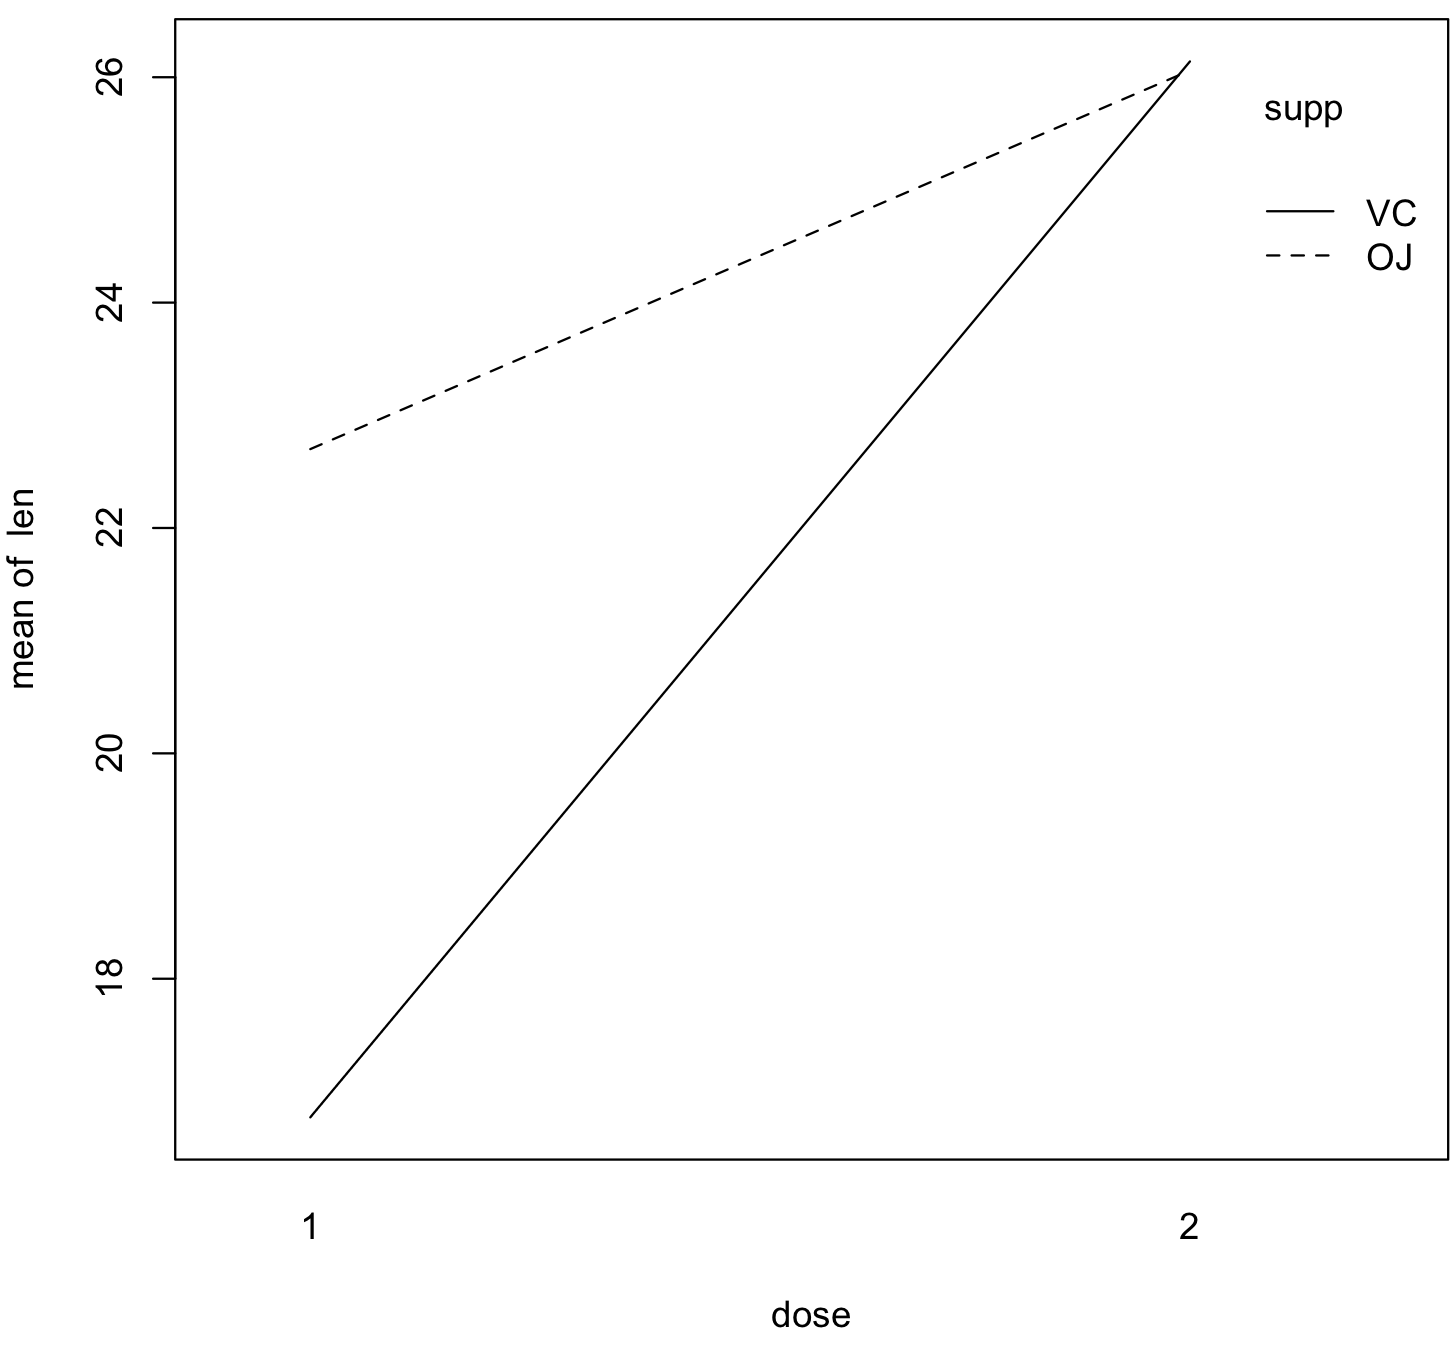
\includegraphics[width=3.3in]{images/toothint2.png}
\end{frame}

\begin{frame}{Interactions}
    \begin{itemize}
        \item There appears to be some interaction between \texttt{dose} and \texttt{supp} 
        \item Recall: an \textbf{interaction} means that the effect of one may partially depend on the value of the other.
        \item We can model this effect by including an additional term:
    \end{itemize}
    \[
        Y = \beta_0 + \beta_1 x_{supp} + \beta_2 x_{dose} + \beta_3 x_{dose} x_{supp} + \epsilon
    \]
\end{frame}

\begin{frame}{Interactions}
    Consider a few rows of the tooth growth data:
    \begin{table}[h]
        \centering
        \begin{tabular}{rrr}
            \hline
            len & supp & dose \\ 
            \hline
            16.5 & VC & 1 \\
            16.5 & VC & 1 \\
            25.5 & VC & 2 \\
            19.7 & OJ & 1 \\
            23.3 & OJ & 1 \\
            26.4 & OJ & 2 \\
            \hline
        \end{tabular}
    \end{table}
    What does this look like with the interaction term?
\end{frame}

\begin{frame}{Example}
    \begin{table}[h]
        \centering
        \begin{tabular}{r rrrr}
            \hline
             & Estimate & Std. Error & t value & Pr$(>|$t$|)$ \\
            \hline
            (Intercept) & 19.3400 & 2.5419 & 7.61 & 0.0000 \\
            suppVC & -11.9400 & 3.5948 & -3.32 & 0.0021 \\
            dose & 3.3600 & 1.6076 & 2.09 & 0.0437 \\
            suppVC:dose & 6.0100 & 2.2735 & 2.64 & 0.0121 \\
            \hline
        \end{tabular}
        \label{tab:my_label}
    \end{table}
    R$^2$: 0.7296, $\quad$ R$^2_{adj}$: 0.7151 
    
    \vspace{12pt}Write out the regression model. Calculate the predicted value for each group. 
\end{frame}

\begin{frame}{Nonlinear Trends}
    \begin{itemize}
        \item One of our regression assumptions is of linear relationships.
        \item What happens when this is violated? 
        \item We may be able to use a \textbf{transformation} to "fix" things.
    \end{itemize}
\end{frame}

\begin{frame}{Transforming the Response Variable}
    These techniques may be useful for violations of
    \begin{itemize}
        \item linearity.
        \item normality of residuals.
        \item constant variability of residuals.
    \end{itemize}
\end{frame}

\begin{frame}{Transformations for Nonlinear Trends}
    We will consider two types of transformation:
    \begin{enumerate}
        \item transforming the response variable.
        \item using polynomial terms in multiple regression.
    \end{enumerate}
\end{frame}

\begin{frame}{Transformations}
    \begin{center}
        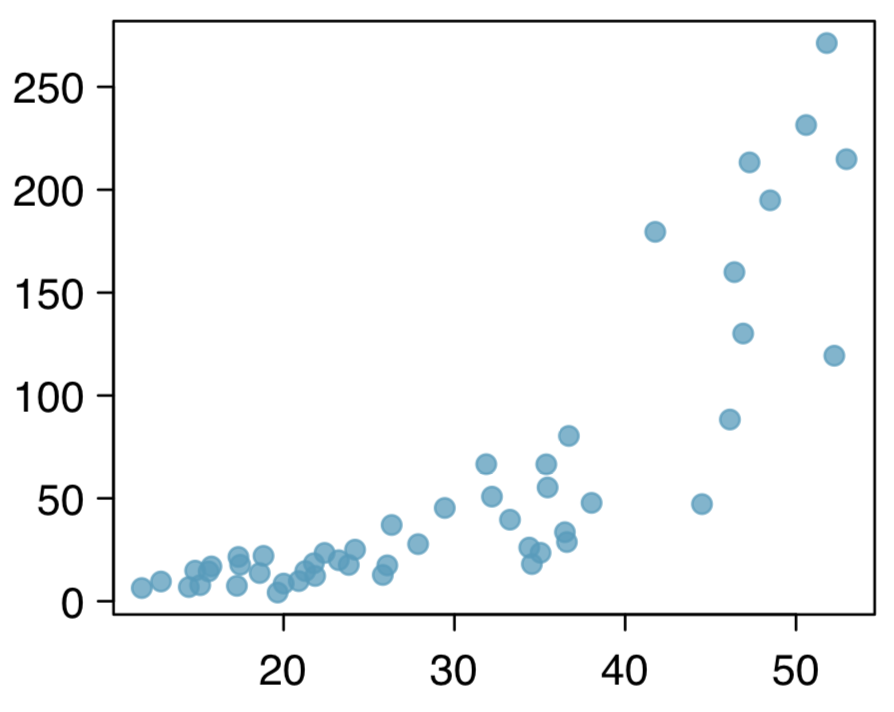
\includegraphics[width=3in]{images/nonlintrend1.png}
    \end{center}
    \vspace{-.75cm}\begin{itemize}
        \item The trend may be nonlinear.
        \item The variability increases with $x$.
    \end{itemize}
\end{frame}

\begin{frame}{Transformations}
    \begin{center}
        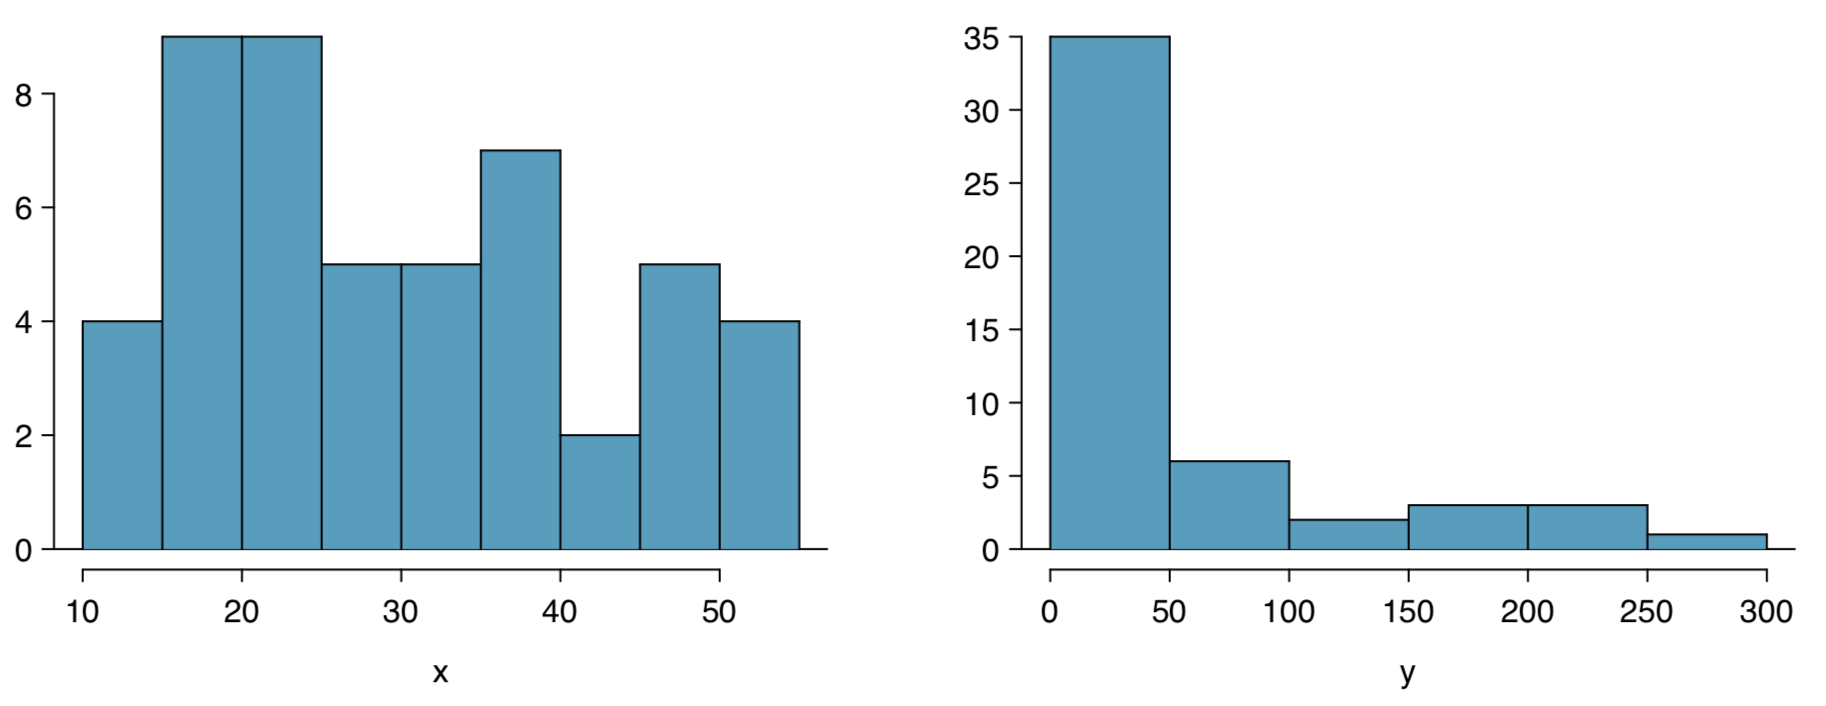
\includegraphics[height=1.75in]{images/histsxy.png}
    \end{center}
    \begin{itemize}
        \item $x$ looks pretty reasonable.
        \item $y$ is extremely right-skewed.
        \item So we probably want to transform $y$.
    \end{itemize}
\end{frame}

\begin{frame}{Transformations on the Response}
    One of the more common transformations is the \textbf{natural log} ($ln$). 
    \[ 
        y^* = \log{y}
    \]
    \vspace{12pt}Note: In statistics, "log" almost always implies the natural log.
\end{frame}

\begin{frame}{Transformations on the Response}
    \begin{center}
        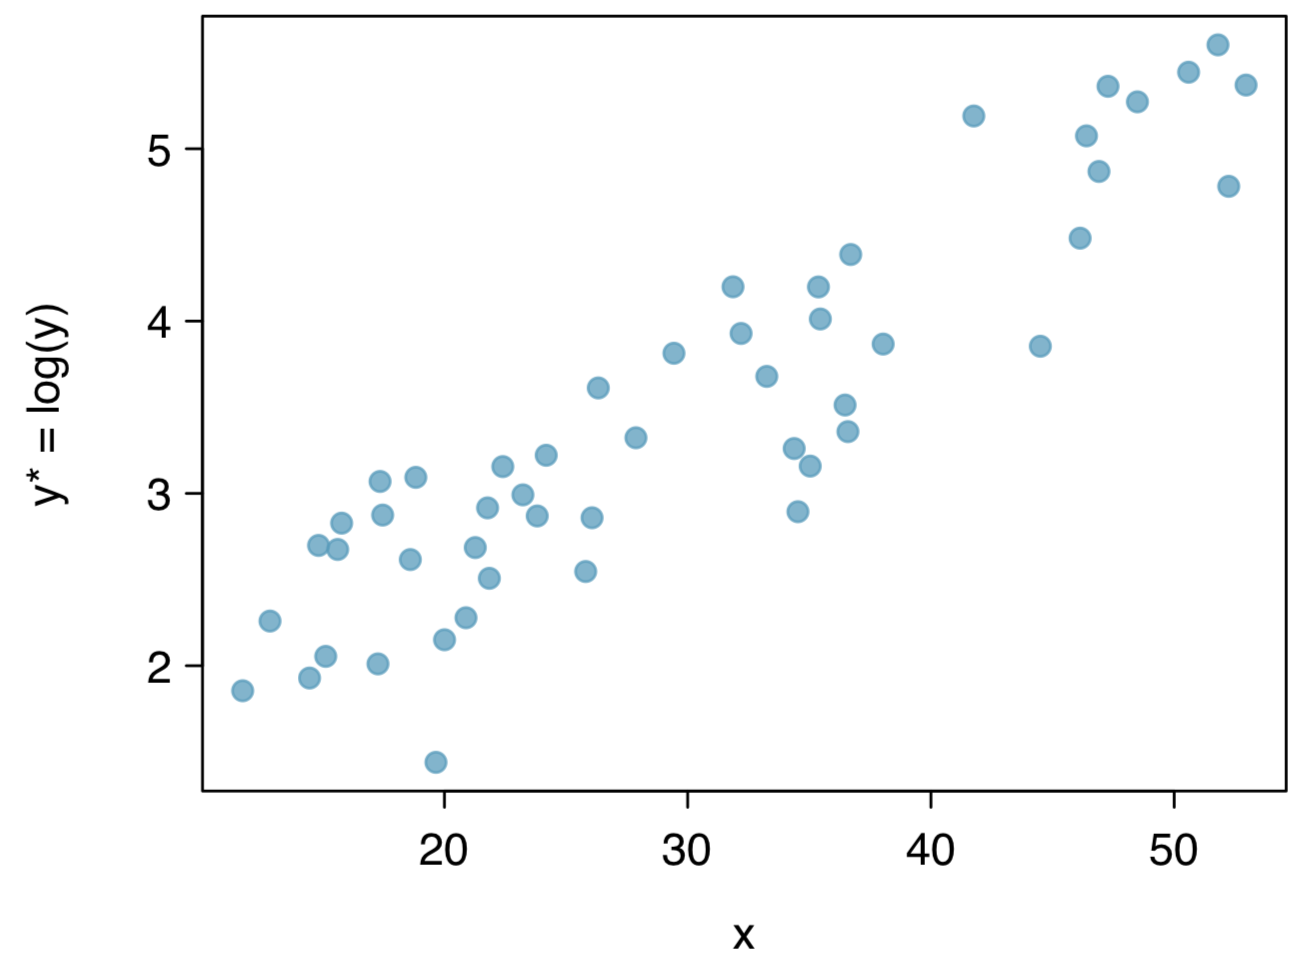
\includegraphics[width=3in]{images/resptrans.png}
    \end{center}
    Now, the relationship looks linear and the variability looks pretty constant.
\end{frame}

\begin{frame}{Back-Transforming}
    The model for these transformed data is
    \[
        \hat{y}^* = 1.03 + 0.08x
    \]
    To get predictions for $y$, we need to \textbf{back-transform} the data by solving for $y$.
    
    \vspace{18pt}Back transform the data and predict the value of $y$ when $x=31$.
\end{frame}

\begin{frame}{Back-Transforming}
    \vspace{-0.5cm}\begin{center}
        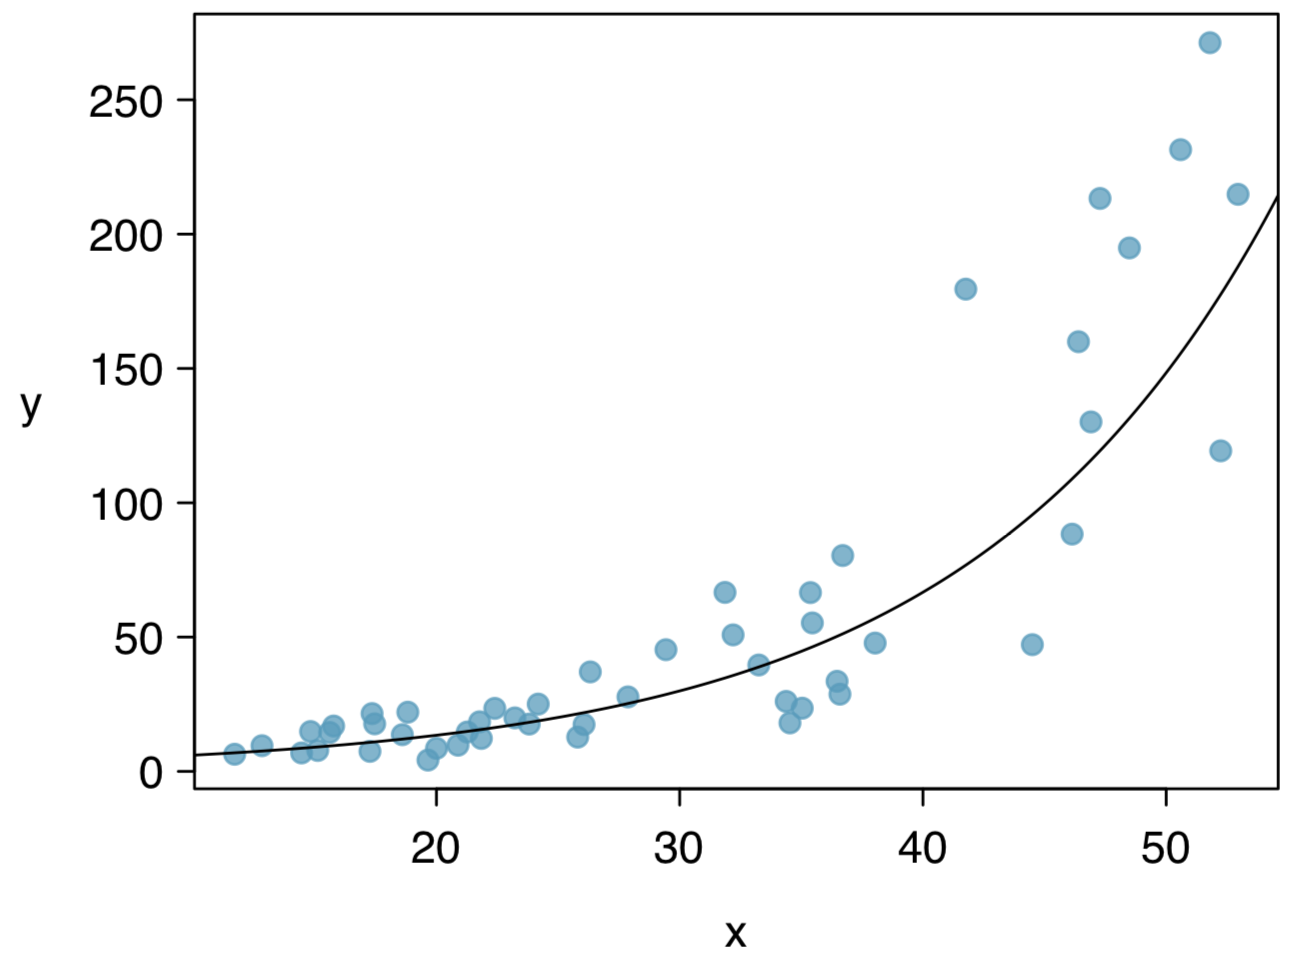
\includegraphics[width=3in]{images/backtran.png}
    \end{center}
    \vspace{-0.5cm}The back-transformed equation overlaid on the original data.
\end{frame}

\begin{frame}{Interpreting Coefficients}
    For a model that used $\log{y}$ and fits the data well, we say
    \begin{itemize}
        \item $y$ tends to grow (or decay) \textbf{exponentially} relative to $x$.
    \end{itemize}
\end{frame}

\begin{frame}{A Word of Caution}
    \begin{itemize}
        \item In theory, there are infinite possible transformations.
        \item If we keep trying different transformations until one "works", we haven't effectively modeled our data.
        \item In actuality, this is a form of data fishing!
        \item This is one reason to think carefully and stick to mostly standard transformations. 
    \end{itemize}
\end{frame}

\begin{frame}{Fitting a Polynomial Curve}
    Consider the following data:
    \begin{center}
        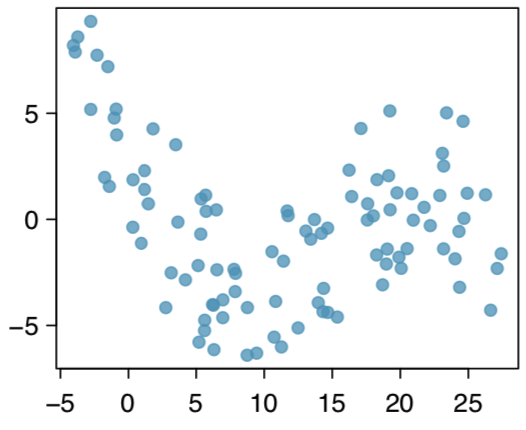
\includegraphics[width=3in]{images/nonlindata2.png}
    \end{center}
\end{frame}

\begin{frame}{Fitting a Polynomial Curve}
    ...with the best fitting straight line:
    \begin{center}
        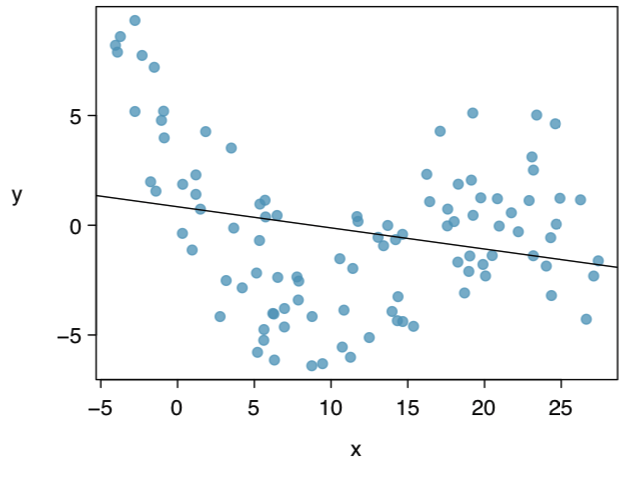
\includegraphics[width=3.5in]{images/nonlindata3.png}
    \end{center}
\end{frame}

\begin{frame}{Fitting a Polynomial Curve}
    \begin{itemize}
        \item Clearly, the straight line does not fit well.
        \item If we drew a curve following the apparent relationship, the variance would be approximately \textbf{homoskedastic}.
        \begin{itemize}
            \item homoskedastic = constant (same) variance
        \end{itemize}
        \item This is a good sign that we want to fit a curve rather than transforming $y$.
    \end{itemize}
\end{frame}

\begin{frame}{Fitting a Polynomial Curve}
    In order to fit a curve, we generate what's called a \textbf{polynomial basis of $\boldsymbol{x}$}.
    
    \vspace{18pt}All this means is that we take $x$ and create
    \begin{itemize}
        \item $x_1 = x$
        \item $x_2 = x^2$
        \item $x_3 = x^3$
        \item etc.
    \end{itemize}
\end{frame}

\begin{frame}{Fitting a Polynomial Curve}
    We will then use these variables in the multiple regression model.
    
    \vspace{12pt}Note:
    \begin{itemize}
        \item It is uncommon to use terms beyond $x^2$.
        \item It is very rare to use terms beyond $x^3$.
    \end{itemize}
\end{frame}

\begin{frame}{The Linear Model}
    Let's start by looking at the best fitting straight line from
    \begin{center}
        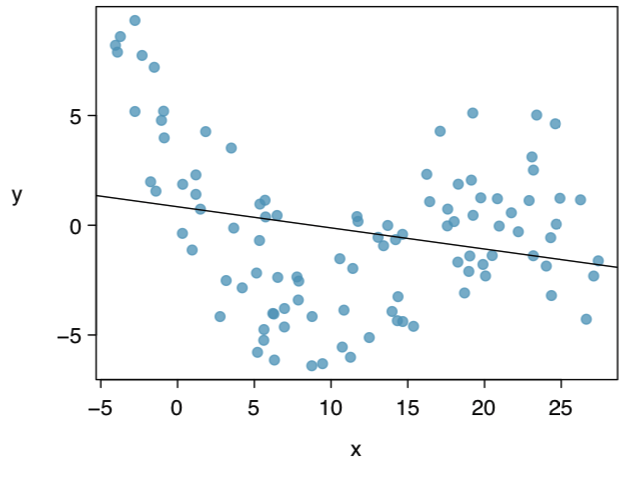
\includegraphics[width=2.5in]{images/nonlindata3.png}
    \end{center}
    \[
        \hat{y} = 0.8441 - 0.0964x
    \]
\end{frame}

\begin{frame}{The Linear Model}
    \begin{table}[h]
        \centering
        \begin{tabular}{r rrrr}
            \hline
             & Estimate & Std Error & t value & Pr$(>|$t$|)$ \\
            \hline
            (Intercept) & 0.8441 & 0.5799 & 1.46 & 0.1487 \\
            x1 & -0.0964 & 0.0397 & -2.43 & 0.0169 \\
            \hline
        \end{tabular}
    \end{table}
    
    Why is this model inappropriate for the data?
\end{frame}

\begin{frame}{Fitting a Polynomial Curve}
    Let's try adding another variable to the model: $x_2 = x^2$.
    
    \begin{itemize}
        \item Generally, when we fit polynomial terms, we include \textit{both variables} in the model.
        \item This is in contrast to a transformation, where we include only the transformed variable.
    \end{itemize}
    
    \[
        y = \beta_0 + \beta_1x_1 + \beta_2x_2 + \epsilon
    \]
\end{frame}

\begin{frame}{Example}
    The model is summarized by
    
    \begin{table}[h]
        \centering
        \begin{tabular}{r rrrr}
            \hline
             & Estimate & Std Error & t value & Pr$(>|$t$|)$ \\
            \hline
            (Intercept) & 2.4252 & 0.5079 & 4.78 & 0.0000 \\
            x1 & -0.7769 & 0.0956 & -8.13 & 0.0000 \\
            x2 & 0.0295 & 0.0039 & 7.55 & 0.0000 \\
            \hline
        \end{tabular}
    \end{table}
    Write out the regression model.
\end{frame}

\begin{frame}{Fitting a Polynomial Curve}
    Based on the scatterplot overlaid with the polynomial curve,
    \begin{center}
        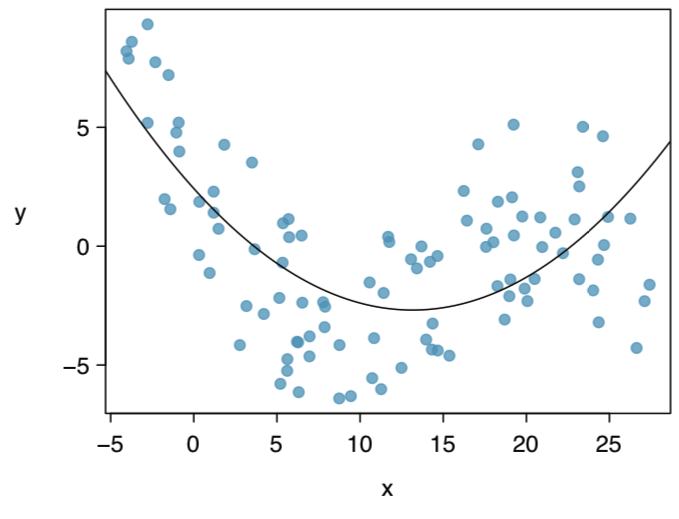
\includegraphics[width=2.5in]{images/nonlindata4.png}
    \end{center}
    a quadratic model is still insufficient.
\end{frame}

\begin{frame}{Cubic Terms}
    Let's try including a cubic term. This model looks like
    \[
        y = \beta_0 + \beta_1x_1 + \beta_2x_2 + \beta_3x_3 + \epsilon
    \]
    where $x_3 = x^3$.
    
    \vspace{12pt}\begin{itemize}
        \item Note that we again include $x_3$ \textit{and} the lower order polynomial terms $x_1$ and $x_2$.
    \end{itemize}
\end{frame}

\begin{frame}{Example}
    This model is summarized by
    
    \begin{table}[h]
        \centering
        \begin{tabular}{r rrrr}
            \hline
             & Estimate & Std Error & t value & Pr$(>|$t$|)$ \\
            \hline
            (Intercept) & 2.0187 & 0.4242 & 4.76 & 0.0000 \\
            x1 & -1.4202 & 0.1236 & -11.49 & 0.0000 \\
            x2 & 0.1187 & 0.0136 & 8.75 & 0.0000 \\
            x3 & -0.0026 & 0.0004 & -6.77 & 0.0000 \\
            \hline
        \end{tabular}
    \end{table}
    Write out the regression model.
\end{frame}

\begin{frame}{Example}
    \begin{center}
        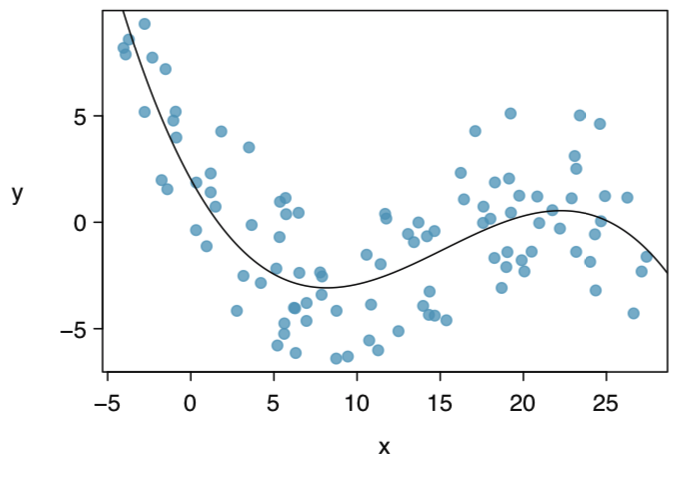
\includegraphics[width=4in]{images/nonlindata5.png}
    \end{center}
\end{frame}

\begin{frame}{Example}
    This model has residual plot
    \vspace{18pt}\begin{center}
        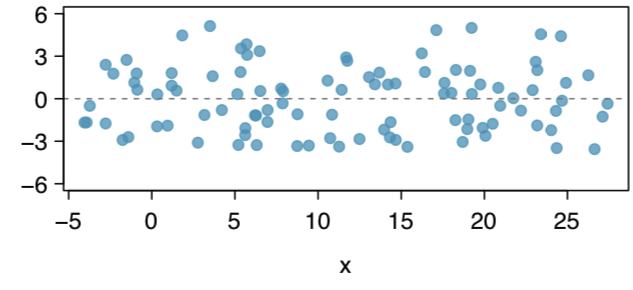
\includegraphics[width=4in]{images/nonlindataresid.png}
    \end{center}
\end{frame}

\begin{frame}{A Word of Caution}
    \begin{itemize}
        \item Start with $x^2$ and use $x^3$ only as necessary.
        \item If a cubic polynomial doesn't work, be very cautious of using higher order polynomials.
        \begin{itemize}
            \item We don't want to force the data to fit!
            \item There are other approaches to modeling that can help deal with this.
        \end{itemize}
        \item Extrapolation is already problematic, but can be much worse for models with transformed data or polynomial terms.
    \end{itemize}
\end{frame}
